\documentclass[tikz,border=10pt]{standalone}
\usepackage{amsmath}
\usetikzlibrary{arrows.meta,positioning,backgrounds,patterns}
\begin{document}
% Shared chapter style: white canvas, sans-serif text, 0.9 pt strokes,
% restrained rounded process boxes, and 3 mm Latex arrowheads.
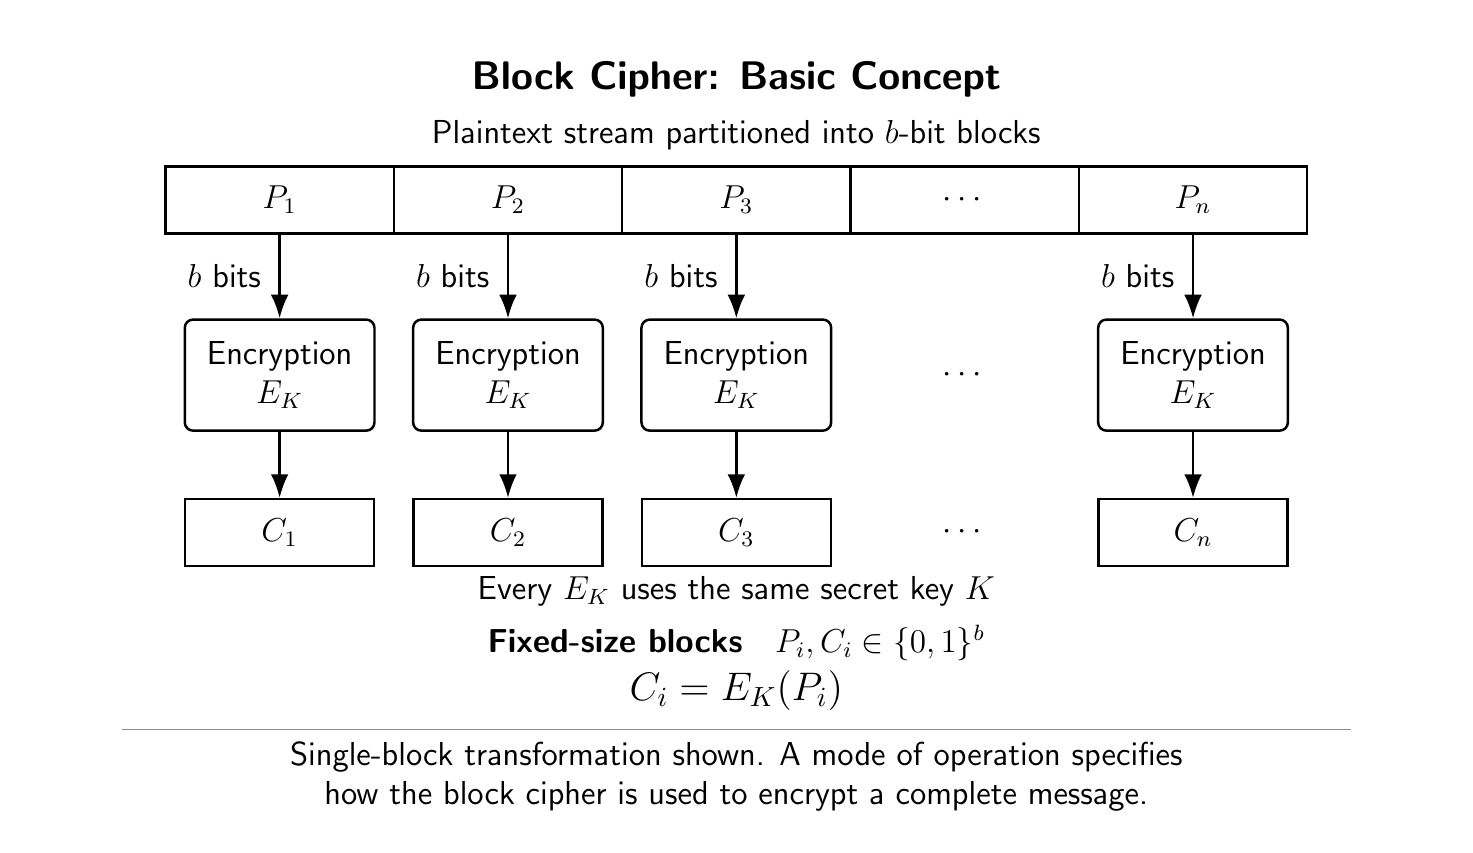
\begin{tikzpicture}[
    font=\sffamily\large, line width=0.9pt,
    background rectangle/.style={fill=white,draw=none},
    show background rectangle,
    box/.style={draw,fill=white,rounded corners=3pt,align=center,inner sep=8pt},
    data/.style={draw,fill=white,align=center,minimum width=2.4cm,minimum height=0.85cm},
    enc/.style={box,minimum width=2.4cm,minimum height=1.05cm},
    arrow/.style={-{Latex[length=3mm]},line width=0.9pt},
    title/.style={font=\sffamily\Large\bfseries,align=center},
    note/.style={align=center},
    repeated/.style={fill=black!14,line width=1.3pt}
]
\path[use as bounding box] (-9,-5.0625) rectangle (9,5.0625);

\node[title] at (0,4.4) {Block Cipher: Basic Concept};
\node[note] at (0,3.7) {Plaintext stream partitioned into $b$-bit blocks};
% A single continuous bar, subdivided into equal-width cells.
\draw[fill=white] (-7.25,2.45) rectangle (7.25,3.3);
\foreach \x in {-4.35,-1.45,1.45,4.35}
    \draw (\x,2.45) -- (\x,3.3);
\foreach \x/\i in {-5.8/1,-2.9/2,0/3,5.8/n} {
    \node (p\i) at (\x,2.875) {$P_{\i}$};
    \node[enc] (e\i) at (\x,0.65) {Encryption\\$E_K$};
    \draw[arrow] (\x,2.45) -- node[left=3pt] {$b$ bits} (e\i.north);
    \node[data] (c\i) at (\x,-1.35) {$C_{\i}$};
    \draw[arrow] (e\i.south) -- (c\i.north);
}
\node at (2.9,2.875) {$\cdots$};
\node at (2.9,0.65) {$\cdots$};
\node at (2.9,-1.35) {$\cdots$};
\node[note,fill=white,inner sep=3pt] at (0,-2.1)
    {Every $E_K$ uses the same secret key $K$};
\node[note] at (0,-2.75)
    {\textbf{Fixed-size blocks}\quad $P_i,C_i\in\{0,1\}^{b}$};
\node[font=\sffamily\Large] at (0,-3.35) {$C_i=E_K(P_i)$};
\draw[black!45,line width=0.6pt] (-7.8,-3.85) -- (7.8,-3.85);
\node[note] at (0,-4.45)
    {Single-block transformation shown. A mode of operation specifies\\
     how the block cipher is used to encrypt a complete message.};
\end{tikzpicture}
\end{document}
